\documentclass[lettersize,journal]{IEEEtran}
% \documentclass[draftcls,onecolumn]{IEEEtran}
\usepackage{amsmath,amsfonts}
\usepackage{algorithmic}
\usepackage{algorithm}
\usepackage{array}
\usepackage[caption=false,font=normalsize,labelfont=sf,textfont=sf]{subfig}
\usepackage{textcomp}
\usepackage{stfloats}
\usepackage{url}
\usepackage{verbatim}
\usepackage{graphicx}
\usepackage{cite}
\usepackage{color}
\usepackage{hyperref}
%\usepackage{subcaption}
% \usepackage{subfigure}
\usepackage{caption}
\usepackage{booktabs}
\usepackage{multirow,makecell}
\usepackage{bm}
\usepackage{amssymb}
\usepackage{amsthm}
\usepackage{adjustbox}
\usepackage{tabularx}
\usepackage{float}
\usepackage[scr=rsfs]{mathalpha}
\usepackage{threeparttable} 
\usepackage{lineno}
\hyphenation{op-tical net-works semi-conduc-tor IEEE-Xplore}
% updated with editorial comments 8/9/2021

\begin{document}
% \pagewiselinenumbers
% \switchlinenumbers
\title{Land cover classification in foggy conditions: Towards Robust Models}

\author{Weipeng Shi, Wenhu Qin$^{*}$, Zhonghua Yun, Allshine Chen, Kai Huang, Tao Zhao
        % <-this % stops a space
\thanks{This work was supported by Key R\&D Program of Jiangsu Province under Grant BE2019311, Jiangsu modern agricultural industry key technology innovation project under Grant CX(20)2013 and
National key research and development program under Grant 
2020YFB160070301. Weipeng Shi\emph{(bowenroom1@gmail.com)}, Wenhu Qin$^{*}$\emph{(corresponding author, qinwenhu@seu.edu.cn)}, Zhonghua Yun, Kai Huang, Tao Zhao are with School of Instrument Science and Engineering, Southeast University, Nanjing, 210096, China. Allshine Chen is with Health Sciences Center, University of Oklahoma, Oklahoma City, 73106, USA.}% <-this % stops a space
}

% The paper headers
\markboth{IEEE Geoscience and Remote Sensing Letters}%
{Weipeng Shi \MakeLowercase{\textit{et al.}}: Land cover classification in foggy conditions: Towards Robust Models}

% \IEEEpubid{0000--0000/00\$00.00~\copyright~2021 IEEE}
% Remember, if you use this you must call \IEEEpubidadjcol in the second
% column for its text to clear the IEEEpubid mark.

\maketitle

\begin{abstract}
Robust semantic labeling of high-resolution remote sensing images in foggy conditions is crucial for automatic monitoring of land covers. This remains a challenging task owing to the low inter-class differentiation yet high intra-class variance and geometric size diversity. Although conventional Convolutional Neural Networks have demonstrated state of the art performance in semantic segmentation, most networks are primarily concerned with standard accuracy, while the influence on robustness is rarely explored. This letter proposes a reliable framework which is evaluated across various severity levels of fog corruptions. Utilizing HRNet as the backbone to maintain high-resolution representations, we develop a multimodal fusion module to exploit the complementary information of lidar and multispectral data. Based on the evaluation experiment on fog corrupted ISPRS 2D datasets, our model demonstrates promising performance with  an average mIoU on the clean along with the corrupted datasets exceeding 80\% and 56\% respectively.

\end{abstract}

\begin{IEEEkeywords}
Semantic segmentation, Attention mechanism, Robust deep learning, Remote sensing, Data fusion
\end{IEEEkeywords}

\section{INTRODUCTION}

Robust semantic segmentation of corrupted remote sensing images (\textbf{RSIs}) means that computer vision models can perform comparatively accurate land cover classification in foggy conditions with minimal performance degradation compared to clean conditions. Fog, which impairs significantly the performance of mineral domain mapping\cite{Lorenz2021FeatureEF}, road extraction \cite{8922802}, 3D reconstruction\cite{9229514}, change detection\cite{6244846}, is often encountered in RSIs. Deep learning based semantic segmentation  models can be summarized into four categories, which are FCNs\cite{shelhamerFullyConvolutionalNetworks2017}, UNets\cite{ronnebergerUNetConvolutionalNetworks2015}, HRNets\cite{wangDeepHighResolutionRepresentation2020} and Visual Transformers\cite{Zheng2021RethinkingSS}. FCNs attain low-resolution representations by serially linking high-to-low convolutions. UNets restore the high-resolution representations through upsampling. HRNets learn ample semantic features with convolution layers in parallel through the multi-resolution fusion units. Visual Transformers have achieved State-of-the-Art (\textbf{SOTA}) results in several vision tasks owing to the powerful modeling capability. SETR\cite{Zheng2021RethinkingSS} proposes a multi-level feature fusion module for fine-grained classification. Segformer\cite{xieSegFormerSimpleEfficient2021} eliminates the time-consuming position encoding module in favor of a lightweight multi-layer perceptron. Additionally,\cite{Zheng2022GeneralizedSC}  possesses both generalization and discrimination abilities through joint learning. For the semantic consistency,\cite{Ning2022SemanticsConsistentRL} considers pairwise and intramodal relationships simultaneously, along with nonpaired intermodal relationships. \cite{Zheng2019ADS} proposes deep scene representation for the context invariance of convolutional neural networks (\textbf{CNN}). 
\begin{figure}[!htbp]
    \centering
    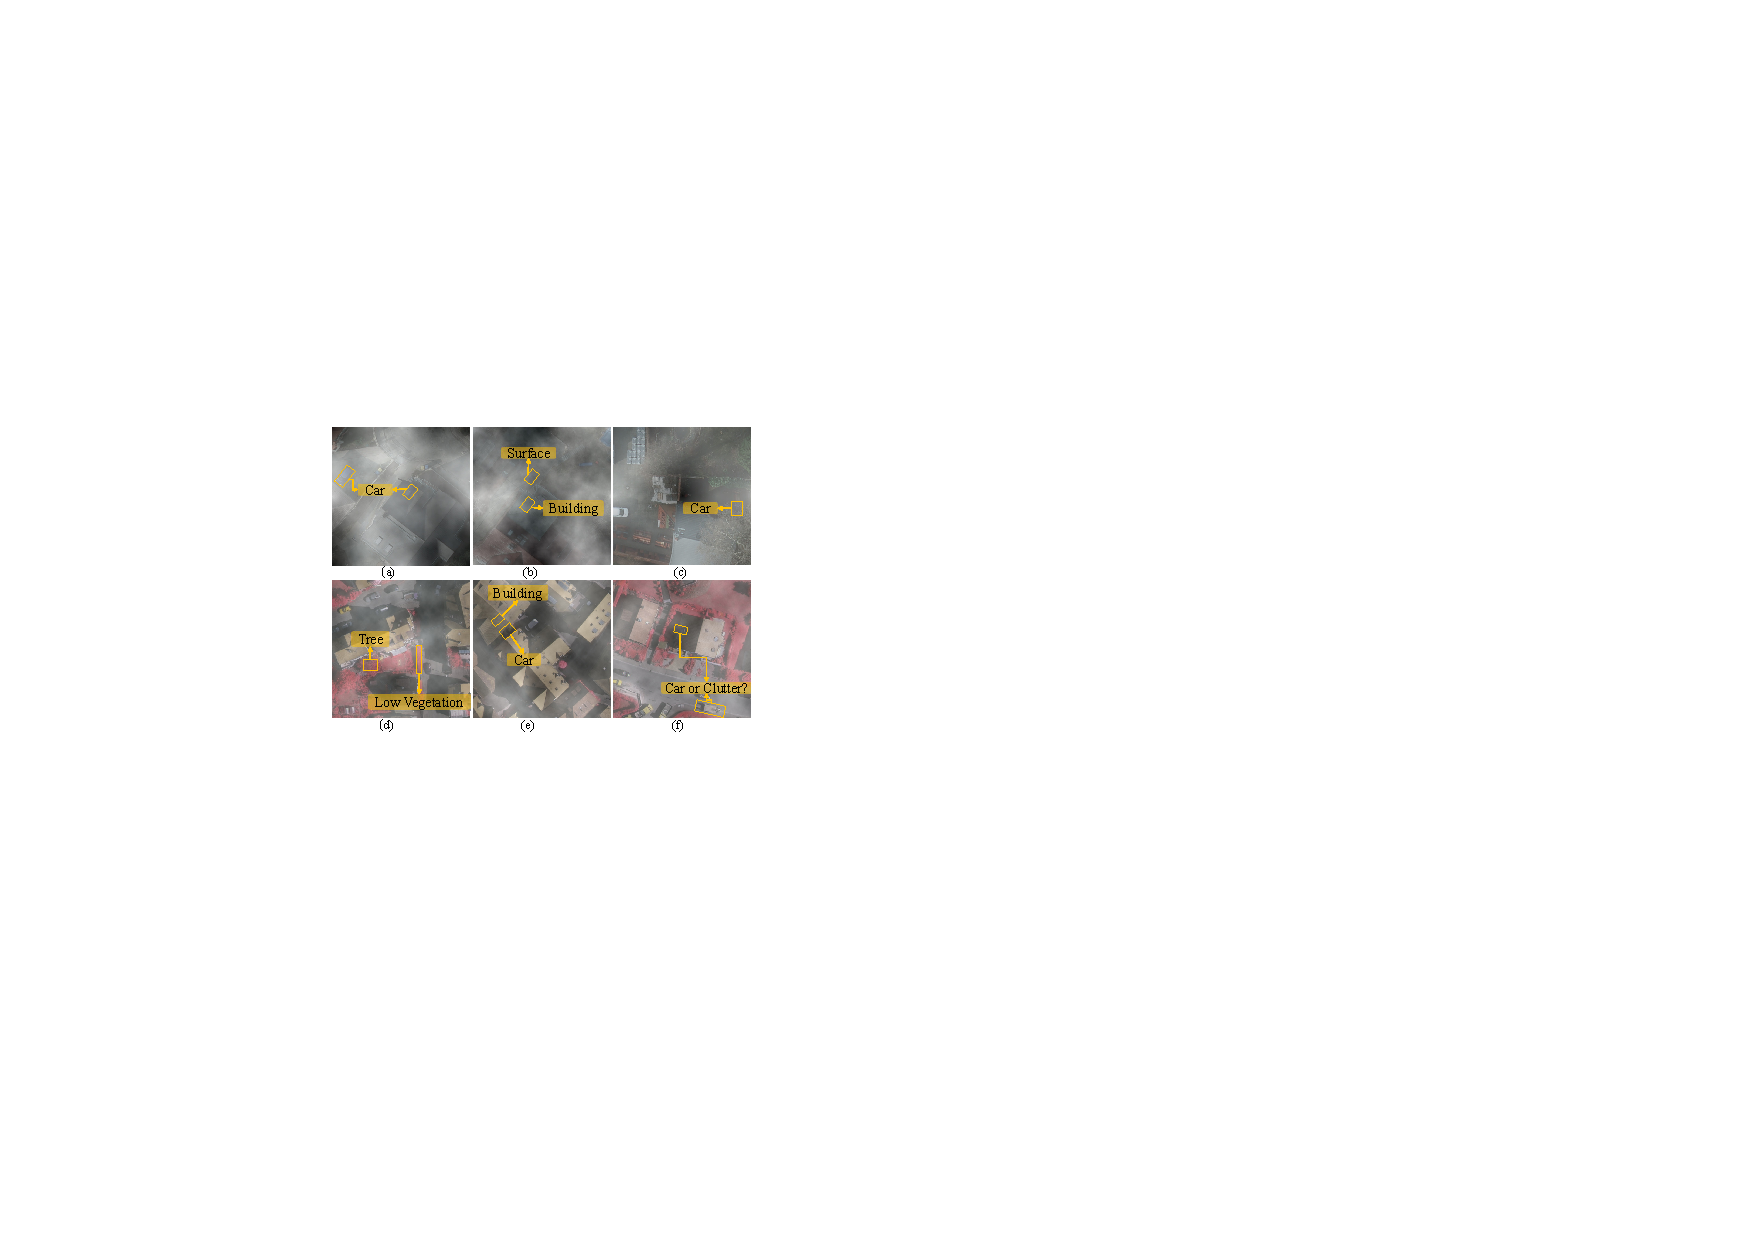
\includegraphics[width=0.9\columnwidth]{challenges.pdf}
    \caption{Challenges associated with robust classification of land covers in fog-covered regions.}
    \label{challenges}
    \vspace{-0.2cm}
\end{figure}

Nonetheless, most semantic segmentation models are trained and validated on natural scene images (\textbf{NSIs}). Previous studies have rarely demonstrated the model's robustness and effectiveness in foggy conditions. Distinct from NSIs, RSIs are of poor quality, which is attributed to the susceptible data acquisition process, particularly when fog exists. Corrupted RSIs pose challenges to robustness, most notably in the following areas:
\begin{itemize}
    \item{\textbf{Intra-class heterogeneity and inter-class homogeneity} Models usually classify objects of the same type into different categories when the shapes and materials differ significantly. In contrast, objects of different classes are occasionally regarded to be identical incorrectly if they share similarities in the appearance. These are intra-class heterogeneity and inter-class homogeneity issues.}
\item{ \textbf{Occlusion and geometric size diversity} Complex 3D interactions exist in RSIs, such as cars parked under the tree shadow or in haze. The accurate classification of spatial relationships cannot be guaranteed by optical cameras alone. Occlusion may lead to large variations in shape and size of objects belonging to the same class. }
\end{itemize}

To alleviate the influence of aforementioned factors associated with remote sensing in foggy circumstances, a framework for robust land cover classification is proposed. HRNet can maintain a consistent high-resolution representation throughout the network. Due to the  adaptability to various scales and shapes, we employ HRNet as the backbone to tackle the intra-class heterogeneity issue. To address occlusion and inter-class homogeneity issues, the proposed multi\-modal fusion module (\textbf{MMF}) investigates the complementary feature maps from the optical input and digital surface model (\textbf{DSM}). Our contributions  can be summarized as follows:
\begin{itemize}
\item We design an end-to-end semantic segmentation model which is robust for land cover classification in foggy conditions.
\item We incorporate MMF into the network leveraging HRNet as a backbone. MMF captures spatial and channel adaptability by utilizing the multimodal remote sensing data efficiently.
\item We conduct experiments on the fog corrupted ISPRS test set to evaluate the effectiveness of our framework.
\end{itemize}
\begin{figure*}[!htbp]
    \centering
    \includegraphics[width=0.73\textwidth]{backbone.pdf}
    \caption{The overall architecture. Our model consists of an encoder (HRNet), a multimodal fusion module and a decoder. In the structure of MMF, \textbf{DW} and \textbf{DW-D} stand for depth-wise convolution and depth-wise dilation convolution, whose kernel sizes are 5 and 7 (dilation rate =3) respectively.}
    \label{backbone}
    \vspace{-0.2cm}
\end{figure*}
\section{METHODOLOGY}
\subsection{Backbone}
Aerial images captured in fog are of poor quality and intra-class heterogeneity is frequently encountered in the process of feature extraction with downsampling. HRNet is adopted as the backbone since it preserves high-resolution representations. The output can acquire rich semantic features without relying on upsampling to recover the high-resolution feature map from the low-resolution.  As illustrated in Fig.\ref{backbone}, HRNet is composed of four separate branches with different resolutions (1/4, 1/8, 1/16, 1/32 of the original). Each branch is further split into four stages, and the output channel numbers are \bm{$C, 2C, 4C, 8C$}. Multi-resolution fusion blocks,  existing between each stage, facilitate information flowing across branches. They are denoted as crossed lines ($3\times 3$ stride convolution and upsampling layer).

All these branches share information with each other on a variety of scales. High-resolution branches focus on spatial details, while lower branches highlight semantic features. HRNet can encode local and spatial information through multi-resolution fusion, acquiring discriminative representations to appropriately classify different objects with the same semantic labeling. This enhances the robustness to intra-class heterogeneity significantly. 


\subsection{Multi-Modal Fusion Module}
Adjacent objects of various classes may exhibit a similar appearance, but owing to different heights, they appear distinctly in DSM, which is advantageous for landscape modeling and visualization. Based on this attribute, we propose MMF for multimodal data fusion, which generalizes well when dealing with occlusion and inter-class homogeneity. We perform grayscale mapping for DSM, which has three channels after the channel replication. According to the conclusion from GCNet\cite{caoGCNetNonlocalNetworks2019},  the gap between feature maps generated by different query locations is narrow, so we design the query independent structure. Originally, the self-attention structure acquires solely the spatial adaptivity, yet it disregards the inter-channel relationship that regularly corresponds to various objects' feature maps. Large convolution kernels provide a large and effective receptive field \cite{guoVisualAttentionNetwork2022}. The optical input contains abundant feature information. Merging with depth-wise \cite{sandlerMobileNetV2InvertedResiduals2019a} model design techniques, we use a large kernel attention to attain long-range dependencies between various channels with the optical input, which is composed of depth-wise convolution(\bm{$K^{DW}$}), depth-wise dilation convolution(\bm{$K^{DW\_D}$}) and $1 \times 1$ convolution(\bm{$K^{1\times 1}$}). MMF can be written as the following:
\begin{equation}
    \mathbf{G}_{k, l, m}=\sum_{i, j} \mathbf{K^{DW}}_{i, j, m} \cdot \mathbf{F^{RGB}}_{k+i-1, l+j-1, m} 
\label{eqDW}   
\end{equation}

\begin{equation}
    \hat{\mathbf{G}}_{k, l, m}=\sum_{i, j} \mathbf{K^{DW\_D}}_{i, j, m} \cdot \mathbf{G}_{k+i-1, l+j-1, m} 
\label{eqDWD}   
\end{equation}

\begin{equation}
    \hat{\mathbf{G}}_{k, l, n}=\sum_{i, j} \mathbf{K^{1\times 1}}_{i, j, m,n} \cdot \hat{\mathbf{G}}_{k+i-1, l+j-1, m} 
\label{eq11}   
\end{equation}
\begin{equation}
    \mathbf{Output} = \hat{\mathbf{G}}_{k, l, n}\otimes \mathbf{F^{DSM}}
\label{eqOutput}   
\end{equation}
 \bm{$F$} $(F\in R^{C\times H \times W})$  and \bm{$G$} are the feature maps. \emph{m, n} indicate the number of input and output channels. Channel numbers of \textbf{F} and \textbf{G} are unified after the depth-wise convolution. As a result of the relatively limited feature information in DSM, we only extract coarse object contextual representations from this input. Depth-wise convolution aims to exploit the relationship between spatial and local areas, whereas dilation convolution is for enlarging the receptive field. $\otimes$ denotes the element-wise product where \bm{$ G_{k, l, n}$} acts as the attention weight for the fusion with DSM input. Therefore, we could explore the multi-modality complementary context from both inputs. 
 \subsection{Decoder}
 We use MLP layers as the decoder, which eliminates the need to design complex components for feature extraction and greatly reduces memory consumption \cite{xieSegFormerSimpleEfficient2021}.  After MLP and upsampling, all the output feature maps \(\mathcal{X} \) (\( \mathcal{X}_{i} \in \mathbb{R}^{\frac{W}{2^{i}} \times \frac{H}{2^{i}} \times C_{i}}\)) from the four branches in HRNet are reduced to 1/4 of the original size, with the identical channel number. Equation.\eqref{eq5} can represent this process, where ${Z_i}$ is the output. 
 \begin{equation}
    {Z_i} = U{P_{(\frac{W}{4},\frac{H}{4})}}({MLP_{v1}}{X_i})
 \label{eq5}
    \end{equation}
\begin{equation}
{Z_2} =  {Conv_{cls}}({MLP_{v2}}(Concat({Z_i})))
\label{eq6}
\end{equation}

Following the concatenation of ${Z_i}$, the fused representation is obtained via $MLP_{v2}$. Finally, the pixel classification is obtained through $1\times 1$  convolution ($Conv_{cls}$). Equation.\eqref{eq6} shows the process for acquiring segmentation mask.

\section{EXPERIMENTS AND ANALYSIS}
\subsection{Dataset}\label{sec:dataset}
The aerial datasets in the experiment originate from Potsdam and Vaihingen provided by ISPRS\footnote{Potsdam and Vaihingen datasets can be acquired from \emph{https://www.isprs.org/education/benchmarks/UrbanSemLab/2d-sem-label-potsdam.aspx} and \emph{https://www.isprs.org/education/benchmarks/UrbanSemLab/2d-sem-label-vaihingen.aspx} (\emph{{Accessed in June, 2022})}}, which have an average resolution of $6000\times 6000$ pixels and $2500\times 2500$ pixels. They consist of cars, low vegetation, buildings, trees, impervious surfaces and cluttered backgrounds. Combining with DSM, RGB and IRRG channel compositions are selected for Potsdam and Vaihingen datasets, respectively. Both are split into the training set, validation set and test set according to the ratio of 0.8, 0.1 and 0.1. We conduct an exploratory analysis and find that cars account for the least, less than 1.7\%. In Vaihingen, 8.57 percent of trees are more prevalent than in Potsdam and other species proportions are comparable. Constrained by the GPU memory, we crop the original high-resolution image into $512\times 512$ and also perform data augmentation, including adjusting image brightness, contrast, rotation, symmetric padding, etc., to reduce overfitting during the training process. 
\begin{figure}[!htbp]
    \centering
    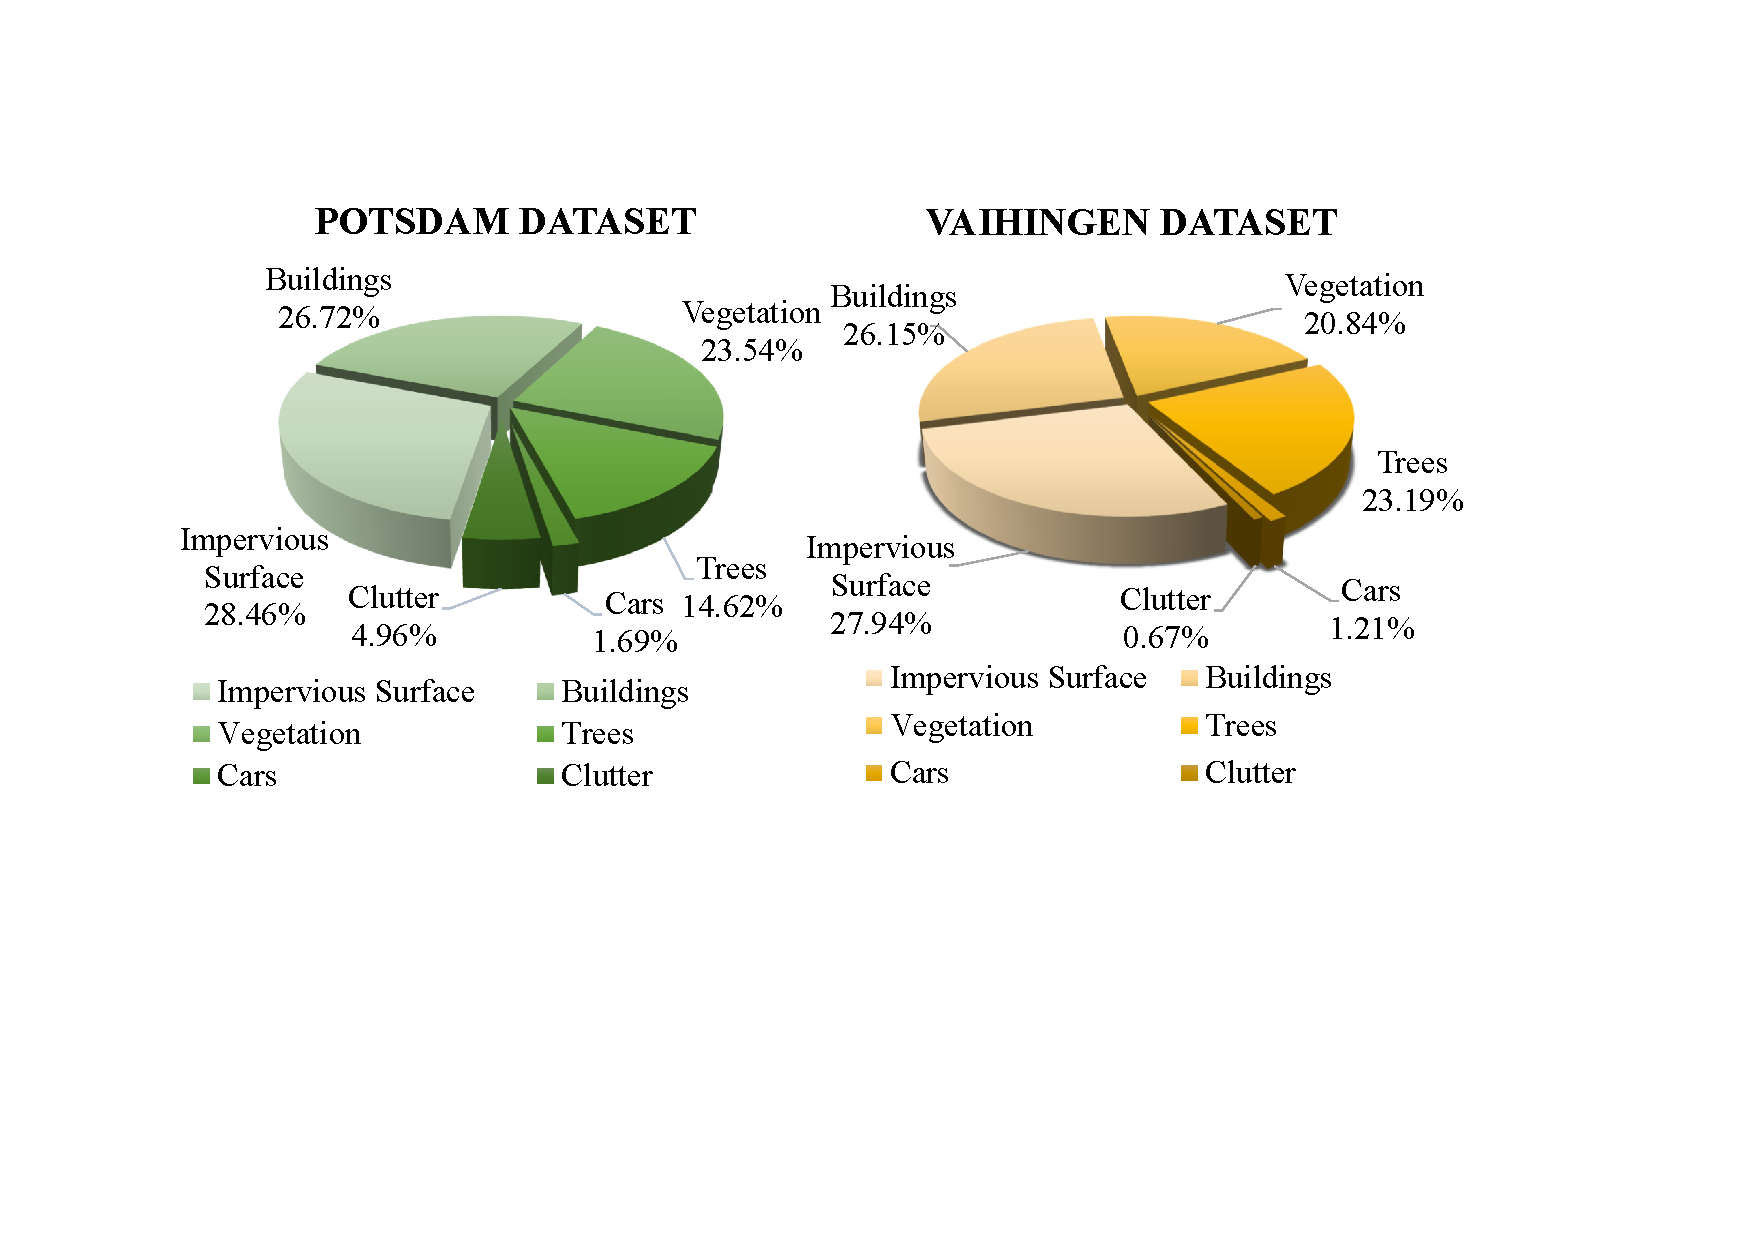
\includegraphics[width=3.5in]{dataset.pdf}
    \caption{Class imbalance exists in both datasets.}
    \label{imbalance}
    \vspace{-0.2cm}
\end{figure}
As can be noted in Fig.\ref{imbalance}, both datasets suffer from the class imbalance issue. Impervious surfaces are approximately sixteen times more numerous than cars. Consequently, there will be a significant bias towards head classes, resulting in the decreased tail class performance. RSIs in ISPRS are captured in normal conditions. To verify that our model is robust in foggy weather, motivated by the robustness evaluation approach in \cite{kamannBenchmarkingRobustnessSemantic2021}, we rendered five different levels of fog for each image in the test set using diamond-square algorithm. Detailed results are shown in Fig.\ref{fogSeverity}. 
       \begin{figure}[!htbp]
        \centering
        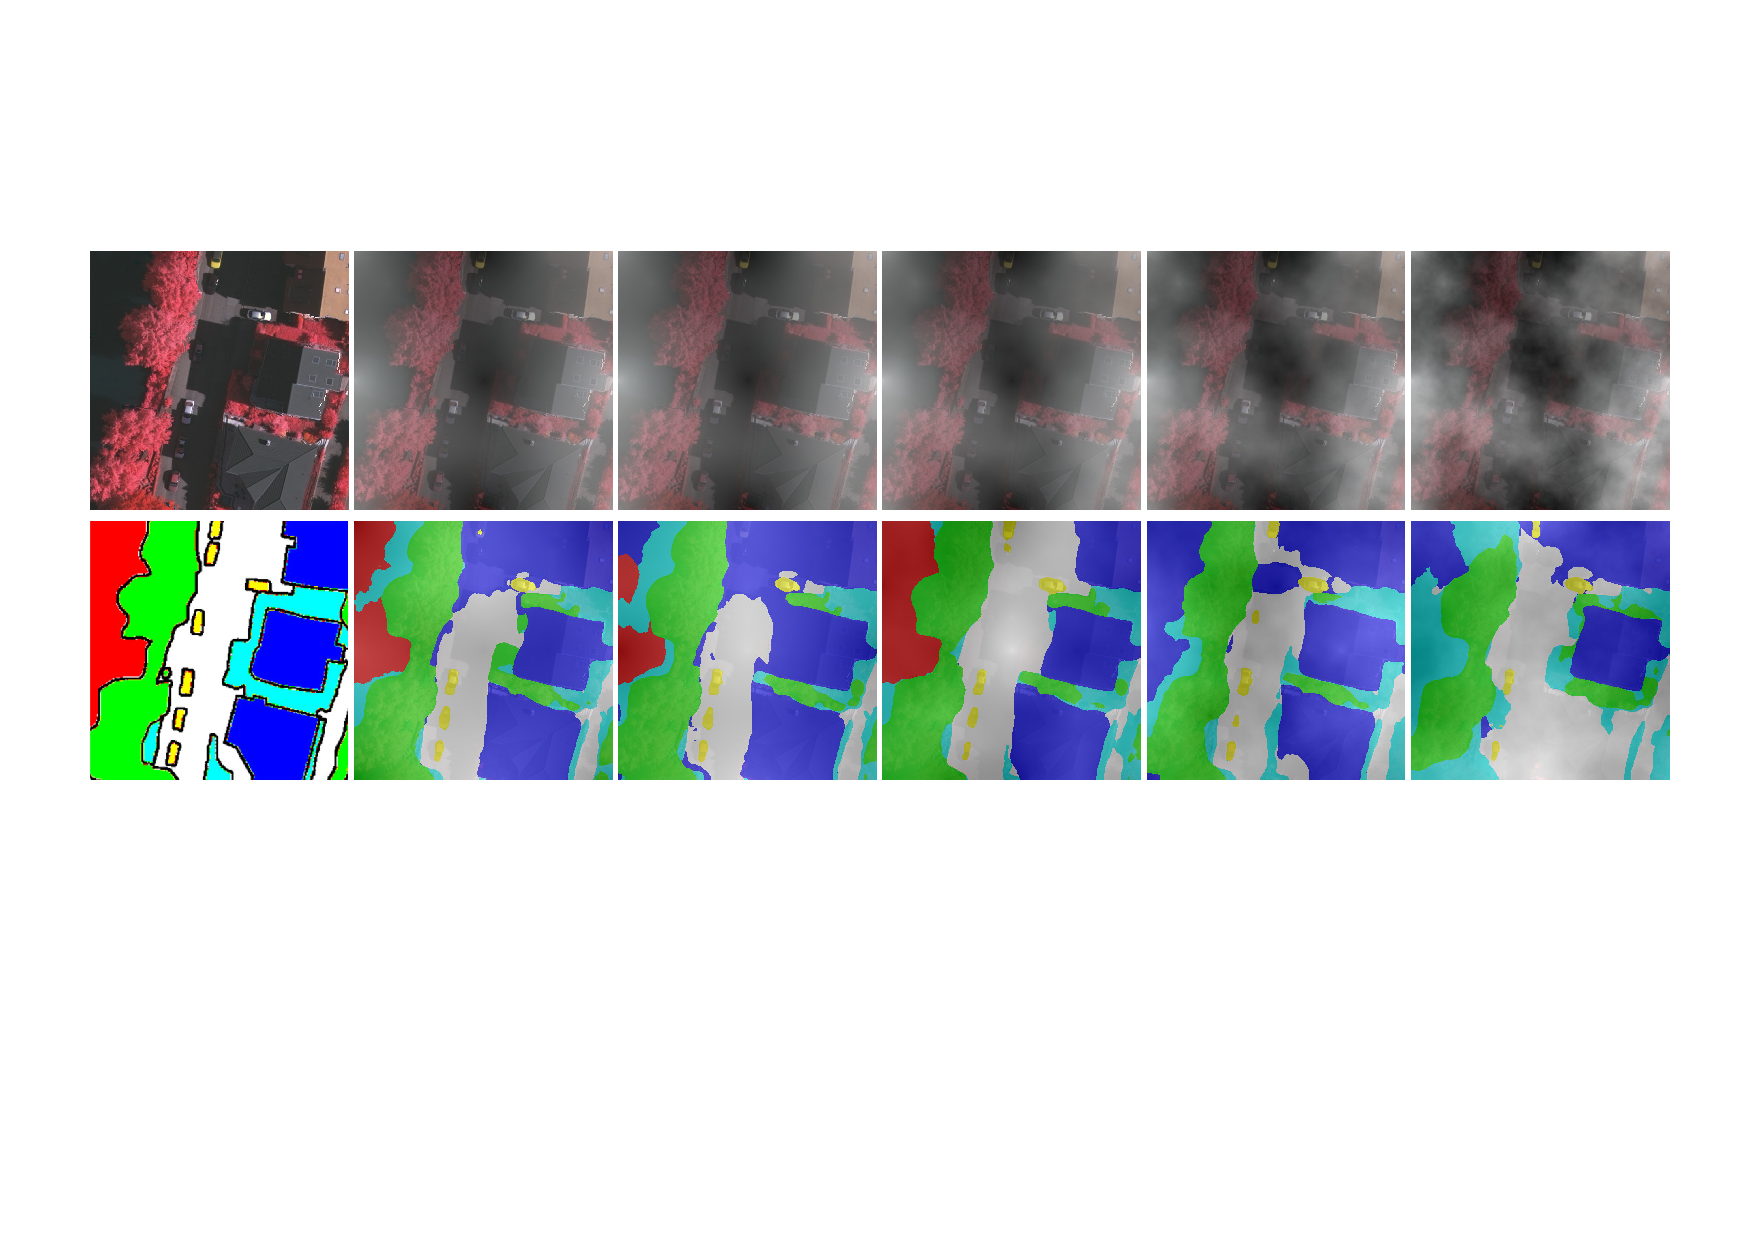
\includegraphics[width=\columnwidth]{fogSeverity}
        \caption{Renderings of five levels of fog severity using Vaihingen dataset. 1st column: clean and ground truth, others: fog of different severity levels with corresponding land cover classification results. }
        \label{fogSeverity}
        \vspace{-0.5cm}
    \end{figure}
\subsection{Metrics}
The evaluation metrics in the experiments are Overall Accuracy (\textbf{OA}), mean Intersection over Union (\textbf{mIoU}) and Corruption Degradation (\textbf{CD}). CD, derived from\cite{kamannBenchmarkingRobustnessSemantic2021}, is the average of degradations across various severity levels which is utilized to evaluate the robustness. Definition of CD is given below:
\begin{small} 
    % \begin{equation}
    %     OA=\frac{T P\ + \ T N}{T P\ +\ F P\ +\ T N \ +\ F N} 
    %     \label{OA}
    % \end{equation}
    % \begin{equation}
    %      I o U= \frac{T P}{F N+F P+T P} 
    %     \label{iou}
    % \end{equation}
    \begin{equation}
        D=1- IoU
        \label{Degradation}
    \end{equation}
    \begin{equation}
         CD^{f}=\frac{\widetilde{D^{f}}}{\widetilde{{D}^{r e f}}}\times 100\% 
        \label{CD}
    \end{equation}
\end{small} 
% True positive, false positive, true negative, and false negative classifications are denoted by  \bm{$TP, FP, TN$} and \bm{$FN$}. 

Higher \textbf{mIoU} and \textbf{OA} values are associated with more accurate land cover classifications. \textbf{ref} and \textbf{f} are the reference and selected model correspondingly. \textbf{D} represents the degradation where $\widetilde{D^{f}}$ stands for the mean degradation acquired across different severity levels of fog corrupted dataset. \textbf{$CD^{f}$} evaluates the absolute robustness performance of method \textbf{f} and the higher portion above 100\% indicates a degradation compared with the reference model in terms of robustness.

\subsection{Implementation Details}
Image with the ID '4-12' in the Potsdam dataset has been removed due to the label error.  All the experiments were conducted on two Titan XP with SyncBN and LayerNorm. We adopt AdamW optimizer and initial learning rate is set to 0. 00006. Poly optimization strategy is adopted with the power and weight decay setting as 1 and 0.01 respectively. Batch size is 10 and we train the model for 288 epochs. For handling class imbalance existing in both datasets, we employ \emph{Unified Focal Loss} \cite{yeungUnifiedFocalLoss2022} function for the robustness and training convergence. 

\subsection{Results and Analysis}
  \emph{Clean} and \emph{Fog} in  Table.\ref{ablatTable}, Table.\ref{compTable} represent the clean and fog corrupted test set respectively.  All the columns except \emph{OA} are \emph{IoU}. The \textbf{higher} the \emph{IoU} of \emph{Clean} and \emph{Fog}, the more accurate the land cover classification will be. Models with \textbf{lower} \emph{CD} perform better in foggy conditions and are more robust than the  reference model.
\begin{table*}[!htbp]
    \LARGE
    \centering
    \caption{ABLATION STUDY ON THE VARIANTS OF VAIHINGEN TEST SET}
    \begin{adjustbox}{width=1\textwidth}
        \begin{tabular}{c|ccc|ccc|ccc|ccc|ccc|ccc|ccc}
            \toprule
            \multirow{2}[4]{*}{\textbf{Method}} & \multicolumn{3}{c|}{\textbf{Imp Surf *}} & \multicolumn{3}{c|}{\textbf{Building}} & \multicolumn{3}{c|}{\textbf{Low Veg *}} & \multicolumn{3}{c|}{\textbf{Tree}} & \multicolumn{3}{c|}{\textbf{Car}} & \multicolumn{3}{c|}{\textbf{mIoU(\%)}} & \multicolumn{3}{c}{\textbf{OA(\%)}} \\
        \cline{2-22}          & \textbf{Clean↑} & \textbf{Fog↑} & \textbf{CD↓} & \textbf{Clean↑} & \textbf{Fog↑} & \textbf{CD↓} & \textbf{Clean↑} & \textbf{Fog↑} & \textbf{CD↓} & \textbf{Clean↑} & \textbf{Fog↑} & \textbf{CD↓} & \textbf{Clean↑} & \textbf{Fog↑} & \textbf{CD↓} & \textbf{Clean↑} & \textbf{Fog↑} & \textbf{mCD↓} & \textbf{Clean↑} & \textbf{Fog↑} & \textbf{CD↓} \\
            \midrule
            \textbf{A: w/o DSM} & 84.30  & 67.18  & 106.59  & 87.79  & 73.29  & 107.92  & 67.76  & 54.79  & 105.19  & 76.34  & 65.26  & 109.35  & 68.99  & 49.15  & 104.80  & 77.04  & 61.93  & 106.77  & 85.07  & 77.87  & 105.73  \\
            \textbf{B: w/o IRRG} & 74.17  & 56.06  & \textbf{142.71 } & 78.55  & 64.95  & \textbf{141.62 } & 54.92  & 48.88  & \textbf{118.94 } & 66.56  & 55.76  & \textbf{139.25 } & 58.16  & 34.24  & \textbf{135.53 } & 66.47  & 51.98  & \textbf{135.61 } & 75.46  & 67.13  & \textbf{157.05 } \\
            \textbf{C: MCC} & 84.31  & 68.42  & 102.57  & 88.55  & 74.35  & 103.64  & 71.32  & 56.93  & 100.21  & \textbf{78.92 } & 67.10  & 103.56  & 70.46  & 50.63  & 101.75  & 78.71  & 63.49  & 102.34  & 87.16  & 78.14  & 104.44  \\
            \textbf{D: w/o MMF} & 83.52  & 66.32  & 109.39  & 86.63  & 71.26  & 116.12  & 67.65  & 52.73  & 109.98  & 75.05  & 64.90  & 110.48  & 67.90  & 41.63  & 120.30  & 76.15  & 59.37  & 113.25  & 85.44  & 77.02  & 109.79  \\
            \textbf{E: Ours} & \textbf{86.36 } & \textbf{69.21 } & 100.00  & \textbf{89.92 } & \textbf{75.25 } & 100.00  & \textbf{72.02 } & \textbf{57.02 } & 100.00  & 78.10  & \textbf{68.23 } & 100.00  & \textbf{70.30 } & \textbf{51.48 } & 100.00  & \textbf{79.34 } & \textbf{64.24 } & 100.00  & \textbf{88.62 } & \textbf{79.07 } & 100.00  \\
            \bottomrule
            \end{tabular}%
          \end{adjustbox}
    \label{ablatTable}%
  \end{table*}%
\begin{table*}[!htbp]
%  \begin{threeparttable}
    \LARGE
        \centering
        \caption{COMPARISON STUDY ON THE VARIANTS OF POTSDAM TEST SET}
        \begin{adjustbox}{width=1\textwidth}
        \begin{tabular}{c|ccc|ccc|ccc|ccc|ccc|ccc|ccc}
            \hline
            \multirow{2}[3]{*}{\textbf{Method}} & \multicolumn{3}{c|}{\textbf{Imp Surf *}} & \multicolumn{3}{c|}{\textbf{Building}} & \multicolumn{3}{c|}{\textbf{Low Veg *}} & \multicolumn{3}{c|}{\textbf{Tree}} & \multicolumn{3}{c|}{\textbf{Car}} & \multicolumn{3}{c|}{\textbf{mIoU(\%)}} & \multicolumn{3}{c}{\textbf{OA(\%)}} \\
        \cline{2-22}          & \textbf{Clean$\uparrow$} & \textbf{Fog$\uparrow$} & \textbf{CD$\downarrow$} & \textbf{Clean$\uparrow$} & \textbf{Fog$\uparrow$} & \textbf{CD$\downarrow$} & \textbf{Clean$\uparrow$} & \textbf{Fog$\uparrow$} & \textbf{CD$\downarrow$} & \textbf{Clean$\uparrow$} & \textbf{Fog$\uparrow$} & \textbf{CD$\downarrow$} & \textbf{Clean$\uparrow$} & \textbf{Fog$\uparrow$} & \textbf{CD$\downarrow$} & \textbf{Clean$\uparrow$} & \textbf{Fog$\uparrow$} & \textbf{mCD$\downarrow$} & \textbf{Clean$\uparrow$} & \textbf{Fog$\uparrow$} & \textbf{CD$\downarrow$} \\
        \cline{1-22}  
            \textbf{FCN\cite{shelhamerFullyConvolutionalNetworks2017}} & 70.08  & 25.64  & \textbf{136.87 } & 71.06  & 37.63  & \textbf{243.54 } & 68.41  & 6.10  & \textbf{105.73 } & 66.72  & 14.24  & \textbf{167.66 } & 41.46  & 13.20  & \textbf{262.95 } & 63.55  & 19.36  & \textbf{183.35 } & 78.41  & 40.76  & \textbf{155.04 } \\
            \textbf{RefineNet\cite{Lin2017RefineNetMR}} & 75.15  & 36.01  & 117.78  & 77.94  & 55.52  & 173.68  & 70.07  & 8.76  & 102.74  & 69.54  & 36.22  & 124.69  & 61.96  & 42.03  & 175.61  & 70.93  & 35.71  & 138.90  & 82.07  & 46.01  & 141.30  \\
            \textbf{DeepLabV3+\cite{chenEncoderDecoderAtrousSeparable2018}} & 76.65  & 37.48  & 115.07  & 78.76  & 64.50  & 138.62  & 72.55  & 9.36  & 102.06  & 69.41  & 40.14  & 117.03  & 58.24  & 49.56  & 152.80  & 71.12  & 40.21  & 125.12  & 82.39  & 49.84  & 131.27  \\
            \textbf{PSPNet\cite{zhaoPyramidSceneParsing2017}} & 78.97  & 35.85  & 118.07  & 76.67  & 61.44  & 150.57  & 73.71  & 9.26  & 102.17  & 68.70  & 38.16  & 120.90  & 61.73  & 47.08  & 160.32  & 71.96  & 38.36  & 130.41  & 80.32  & 47.26  & 138.03  \\
            \textbf{SETR\cite{zhengRethinkingSemanticSegmentation2021a}} & 76.45  & 37.44  & 115.15  & 75.44  & 62.03  & 148.26  & 70.65  & 10.20  & 101.11  & 69.69  & 40.49  & 116.34  & 62.16  & 52.58  & 143.65  & 70.88  & 40.55  & 124.90  & 85.03  & 50.06  & 130.70  \\
            \textbf{OCRNet\cite{yuanSegmentationTransformerObjectContextual2021} } & 78.24  & 44.21  & 102.69  & 85.50  & 69.81  & 117.88  & 74.67  & \textbf{11.41 } & 99.75  & 73.49  & 46.12  & 105.34  & 76.14  & 63.22  & 111.42  & 77.61  & 46.95  & 107.42  & 87.67  & 58.50  & 108.61  \\
            \textbf{Segmenter\cite{strudelSegmenterTransformerSemantic2021}} & 77.77  & 40.50  & 109.52  & 82.88  & 55.09  & 175.36  & 71.76  & 9.24  & 102.20  & 72.92  & 40.36  & 116.60  & 74.25  & 51.45  & 147.08  & 75.92  & 39.33  & 130.15  & 83.70  & 49.45  & 132.30  \\
            \textbf{SegFormer\cite{xieSegFormerSimpleEfficient2021}} & 78.85  & 42.81  & 105.26  & 84.33  & 70.73  & 114.29  & 72.72  & 11.03  & 100.18  & 72.89  & 45.41  & 106.73  & 75.96  & 62.55  & 113.45  & 76.95  & 46.51  & 107.98  & 87.43  & 56.22  & 114.58  \\
            \textbf{Ours} & \textbf{84.20 } & \textbf{45.67 } & 100.00  & \textbf{89.92 } & \textbf{74.39 } & 100.00  & \textbf{74.54 } & 11.19  & 100.00  & \textbf{77.94 } & \textbf{48.85 } & 100.00  & \textbf{80.19 } & \textbf{66.99 } & 100.00  & \textbf{81.36 } & \textbf{49.42 } & 100.00  & \textbf{89.25 } & \textbf{61.79 } & 100.00  \\
            \hline
            \end{tabular}%
        \end{adjustbox}
        \label{compTable}%
%    \end{threeparttable}% 
\end{table*}
\subsubsection{Ablation Study}

\begin{table}[htbp]
    \centering
    \caption{Various backbones on corrupted Vaihingen test set}
      \begin{tabular}{cccc}
      \toprule
      \textbf{Backbone} & \textbf{mIoU(\%)↑} & \textbf{OA(\%)↑} & \textbf{CD(\%)↓} \\
      \midrule
      ResNet-101 & 51.45  & 70.88  & 135.77  \\
      ResNext-101 & 57.64  & 72.06  & 118.46  \\
      MiT-B5 & 61.28  & 77.10  & 108.28  \\
      MobileNetV2 & 47.10  & 65.85  &  \textbf{147.93}  \\
      HRNet-W48 &  \textbf{64.24} & \textbf{79.07} & 100.00  \\
      \bottomrule
      \end{tabular}%
    \label{backboneTab}%
  \end{table}%
  
  To verify the effectiveness of the backbone, an ablation study was conducted using fog corrupted test set. The backbone in Fig.\ref{backbone} was replaced with ResNet-101, ResNext-101,MiT-B5\cite{xieSegFormerSimpleEfficient2021}, MobileNetV2\cite{sandlerMobileNetV2InvertedResiduals2019a}, HRNet-W48\cite{wangDeepHighResolutionRepresentation2020}. As can be concluded from Table.\ref{backboneTab}, MobileNetV2 has inferior classification accuracy and robustness  in view of a small number of parameters. Mit-B5 shows a relatively better performance in robustness when fog exists. HRNet-W48 demonstrates a 2.96\% improvement in mIoU along with a 8.28\% reduction in CD over MiT-B5.
  \begin{figure}[!htbp]
    \centering
    % \includegraphics[width=0.8\columnwidth]{dataPlot}
    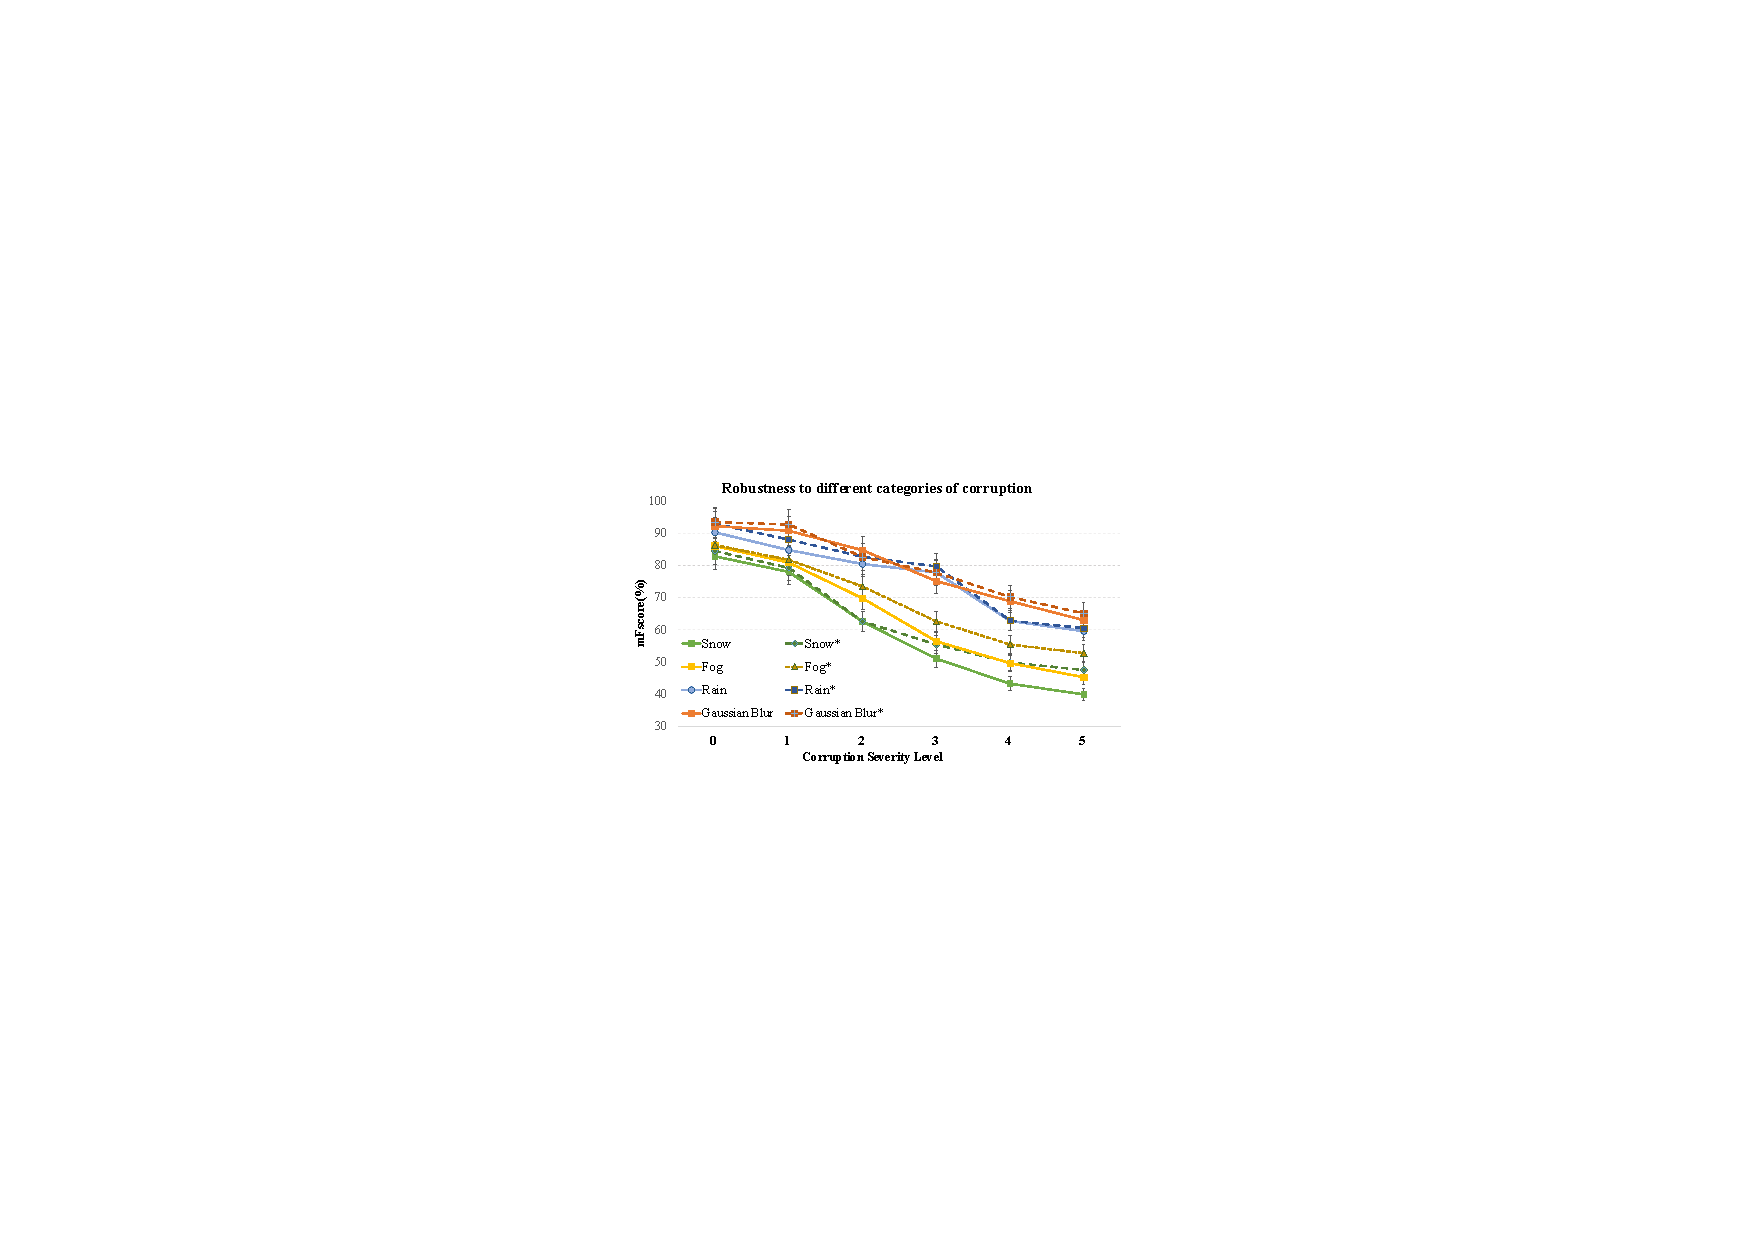
\includegraphics[width=3.5in]{dataPlot2}
    \caption{Ablation study visualization on fog corrupted Vaihingen test set. In the radar plot, a smaller envelop indicates better robustness. Increasing fog severity shows mIoU degradation.}
    \label{dataPlot}
    \vspace{-0.5cm}  
    \end{figure}

To validate the effectiveness of each element, we conduct an ablation study on the Vaihingen dataset and results are shown in Table. \ref{ablatTable} and Fig.\ref{dataPlot}. \textbf{w/o} in Table. \ref{ablatTable} represents \textbf{without}, w/o DSM along with w/o IRRG represent we only use the data from the same modality with identity mapping, thus verifying that model can learn the complementary relationship from multi-modal inputs to enhance the robustness. \textbf{MCC} represents replacing MMF with multi-channel concatenation, thereby testing whether pure channel stacking or MMF is better at fusing multi-modal data. w/o MMF indicates replacing  MMF with $1\times 1$ convolution and sum operations. Our model is set as the reference. From the comparison of A and B in Table. \ref{ablatTable}, it is worth noting that mIoU performance on the clean data of DSM has decreased by 10.57\% due to the lack of IRRG. mCD, which increases by 28.84\%, demonstrates the degradation of robustness without IRRG during training. Looking into the results A, B and C, multi-modality outperforms the single one in mIoU by nearly 2\%. Observing C and E, MMF will bring a decrease in mCD of 2.34\%. The comparison between D and E indicates that MMF is more effective at obtaining the complementary characteristics of multimodality than $1\times 1$ convolution. There will be an almost 10\% and 3\% improvement in robustness and accuracy, respectively. 

The right panel in Fig.\ref{dataPlot} demonstrates the performance on the corrupted Vaihingen dataset with different severity levels of fog.  \emph{Level0} denotes the clean dataset. Model trained only on the DSM input has the worst robustness.  The difference between each method is not significant when the corruption degree is within 1$\thicksim $ 3. Models with MMF and MCC are characterized with better performance in both accuracy and robustness. 


\begin{figure}[!htbp]
    \centering
    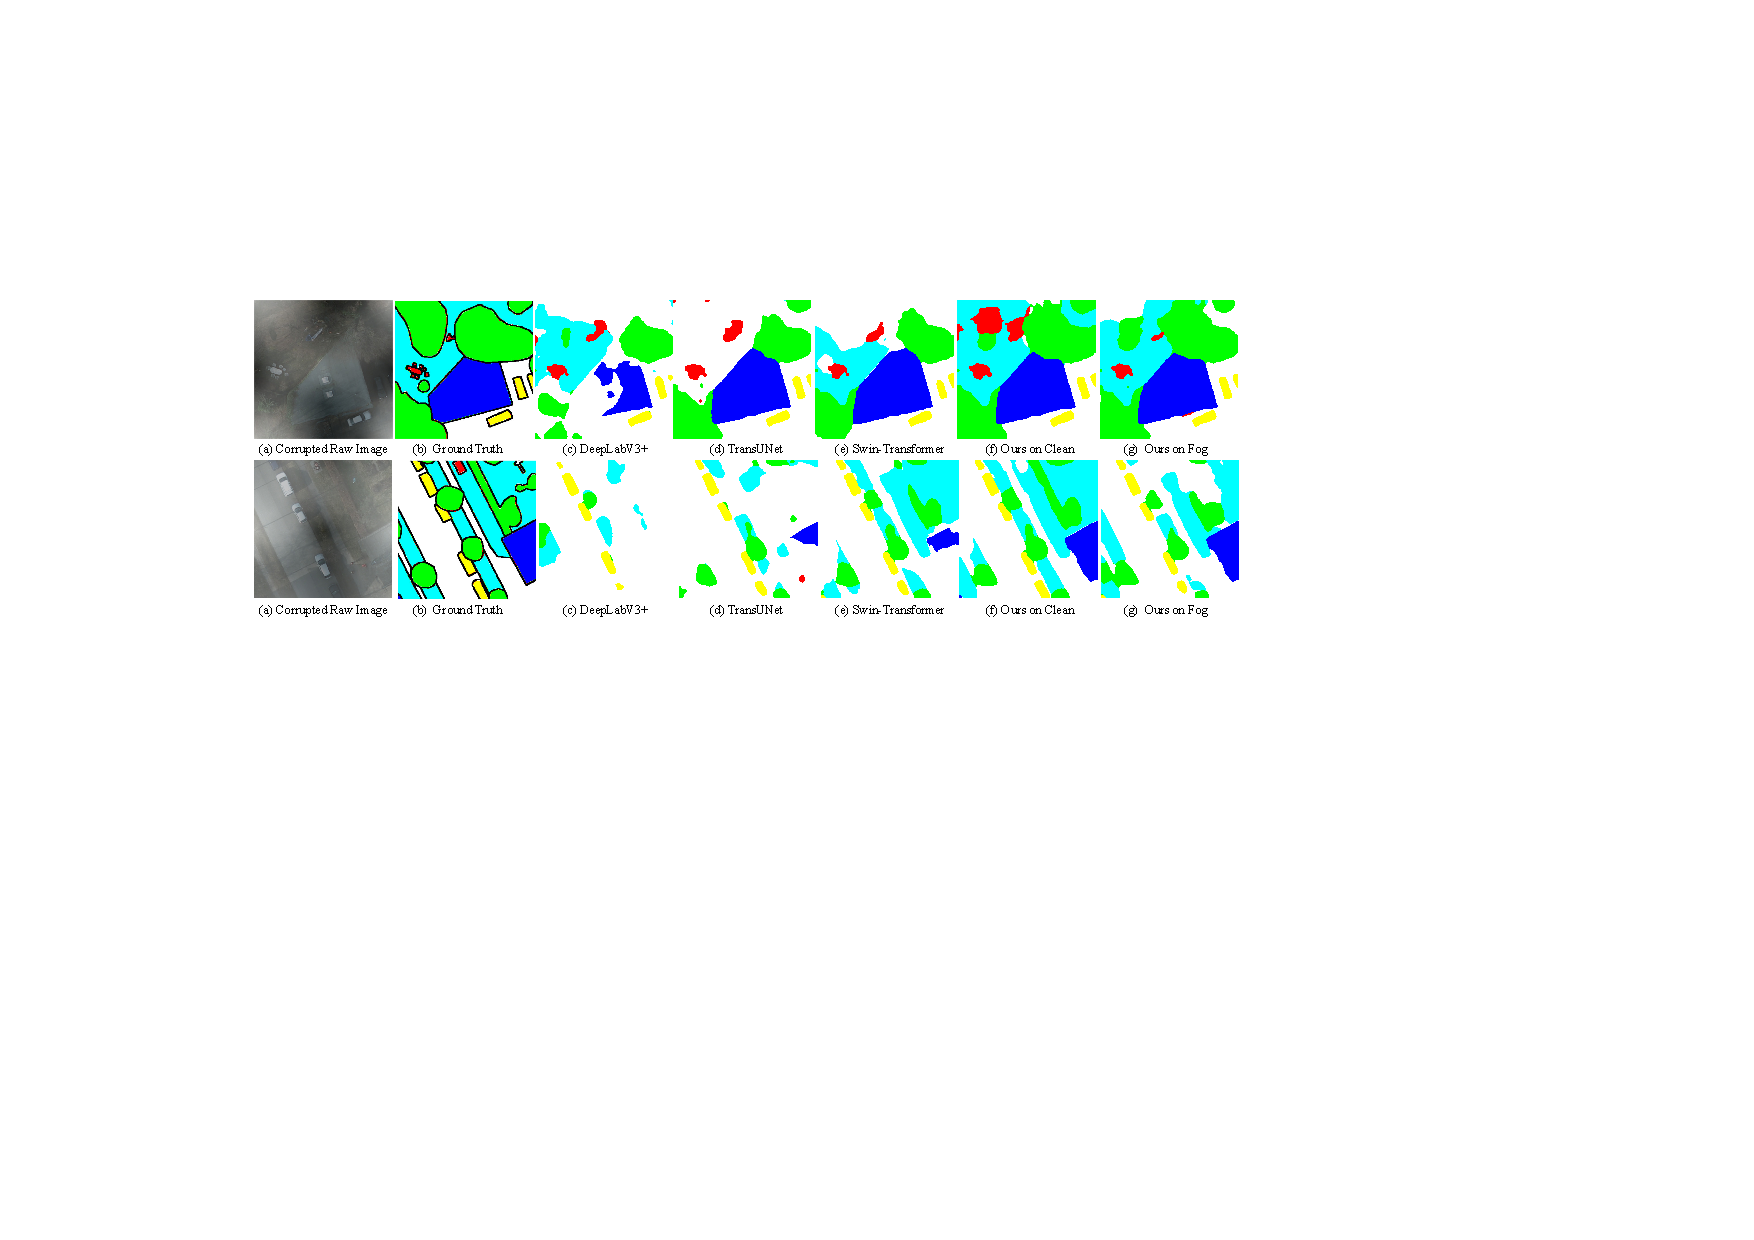
\includegraphics[width=\columnwidth]{visualResult.pdf}
    \caption{Qualitative comparisons of several approaches for semantic segmentation of RSIs. The original image is corrupted by the fog of severity level three.
}
    \label{visualResult}
    \vspace{-0.5cm}  
\end{figure}

\subsubsection{Comparison Study}

      To compare the performance of different methods, we conducted a comparison study on the Potsdam test set. The selected methods can be separated into two groups: CNN-based models whose backbone is ResNet101 (including FCN \cite{shelhamerFullyConvolutionalNetworks2017}, RefineNet \cite{Lin2017RefineNetMR}, DeepLabV3+ \cite{chenEncoderDecoderAtrousSeparable2018}, PSPNet \cite{zhaoPyramidSceneParsing2017}, OCRNet \cite{yuanSegmentationTransformerObjectContextual2021}) and Transformer-based models (like SETR \cite{zhengRethinkingSemanticSegmentation2021a}, Segmenter \cite{strudelSegmenterTransformerSemantic2021}, and Segformer \cite{xieSegFormerSimpleEfficient2021} using DeiT-B, DeiT-B and MiT-B5 \cite{xieSegFormerSimpleEfficient2021} as the backbone). The number of parameters is approximately 70-90M for each model. In all cases except ours, the input multimodal data are concatenated over one dimension. It can be observed from Table.\ref{compTable} that OCRNet perform best excluding ours. Our model, compared to OCRNet, delivers a 3.75\% and 2.47\% improvement in mIoU performance on \emph{Clean} and \emph{Fog} respectively, as well as a 7.42\% reduction in mCD. In terms of robustness to natural corruption noises, Transformers perform worse than CNNs due to the requirement of large amount of data for pre-training.  The inference result on corrupted image (a) under severity level 3 is illustrated in Fig.\ref{visualResult}. Model that is sensitive to natural noise, such as (c) (d) (f), cannot classify trees and low vegetation accurately as a result of dense fog in the box area. Ours can well capture the long-range dependencies, not only can precisely label the objects in the box area, but also facilitate fine-grained classification of the edges.  Our model shows superior robustness and an improvement in the land cover classification of fog corrupted scenes comparing to previous ones.

\section{CONCLUSION}
In this letter, we propose an end-to-end robust framework for the classification of land covers. Based on HRNet, we show that complementary features from multi-modality fusion can be learned by MMF to improve robustness performance.
Experiment results indicate that our model generalizes well on the fog corrupted test set and achieves a balance between accuracy and robustness. We hope that this letter will motivate scholars and practitioners in this area to further investigate how to design a robust model in the remote sensing domain.

%  \newpage
\bibliography{IGRLRef}
\bibliographystyle{IEEEtran.bst}
 
\end{document}


